% Created 2022-10-17 lun 09:02
% Intended LaTeX compiler: pdflatex
\documentclass[12pt]{article}
\usepackage[utf8]{inputenc}
\usepackage[T1]{fontenc}
\usepackage{graphicx}
\usepackage{grffile}
\usepackage{longtable}
\usepackage{wrapfig}
\usepackage{rotating}
\usepackage[normalem]{ulem}
\usepackage{amsmath}
\usepackage{textcomp}
\usepackage{amssymb}
\usepackage{capt-of}
\usepackage{hyperref}
\usepackage[spanish]{babel}
\usepackage{graphicx,geometry}
\geometry{ a4paper, left=1in, right=1in, top=1in, bottom=1in }
\renewcommand\familydefault{\sfdefault}
\usepackage{sectsty}
\sectionfont{\normalfont\Large }
\subsectionfont{\normalfont}
\usepackage{tabularx}
\usepackage{listings}
\lstdefinestyle{mystyle}{
numbers=left,
showspaces=false,
frame=leftline,
showspaces=false,
showstringspaces=false,
showtabs=false,
numberstyle=\tiny,
}
\lstset{
style=mystyle,
literate={á}{{\'a}}1
{é}{{\'e}}1
{í}{{\'{\i}}}1
{ó}{{\'o}}1
{ú}{{\'u}}1
{Á}{{\'A}}1
{É}{{\'E}}1
{Í}{{\'I}}1
{Ó}{{\'O}}1
{Ú}{{\'U}}1
{ü}{{\"u}}1
{Ü}{{\"U}}1
{ñ}{{\~n}}1
{Ñ}{{\~N}}1
{¿}{{?``}}1
{¡}{{!``}}1
}
\makeatletter
\usepackage{fancyhdr}
\pagestyle{fancy}
\usepackage{mdframed}
\BeforeBeginEnvironment{minted}{\begin{mdframed}}
\AfterEndEnvironment{minted}{\end{mdframed}}
\author{Luis Eduardo Galindo Amaya (1274895)}
\date{14-10-2022}
\title{Instrucciones, lógicas y de manipulación de bits.}
\hypersetup{
 pdfauthor={Luis Eduardo Galindo Amaya (1274895)},
 pdftitle={Instrucciones, lógicas y de manipulación de bits.},
 pdfkeywords={},
 pdfsubject={},
 pdfcreator={Emacs 26.3 (Org mode 9.1.9)}, 
 pdflang={Spanish}}
\begin{document}



\newcommand{\docente}{Arturo Arreola Alvarez}
\newcommand{\asignatura}{Organización de Computadoras (331)}
\newcommand{\semestre}{2022-2}

\newcommand{\miportada}[1]{
	\begin{titlepage}
		\vspace*{0.75in}
		\begin{flushleft}
			\sffamily
			\large #1       \\
			\Huge 
            \@title         \\
			\hrulefill
			\vspace{0.25in} \\
			\Large \@author \\
			\vspace*{\fill}
            
\includegraphics[width=\textwidth]{../includes/filler.png} \\
			\vspace*{\fill}
			\large
			\begin{tabular}{|l|l|}
              \hline
			  Asignatura & \asignatura \\
			  Docente    & \docente    \\
			  Fecha      & \@date      \\
              \hline
			\end{tabular}
		\end{flushleft}
	\end{titlepage}
}

\miportada{ Práctica 8 }

\fancyhf{}
\lhead{ \asignatura }
\rhead{ \semestre }
\rfoot{Página \thepage}

\setlength\parindent{0pt}   % eliminar el intentado
\setlength{\parskip}{1.2em}
\maketitle

\section*{Objetivo}
\label{sec:org3175bb2}
Seleccionar las instrucciones lógicas y de manipulación de bits adecuadas
para desarrollar aplicaciones de sistemas basados en microprocesador
mediante la distinción de su funcionamiento, de forma lógica y ordenada.

\section*{Desarrollo}
\label{sec:orgd677130}
\subsection*{Parte 1}
\label{sec:org28ec5b1}
Descargue el archivo print\_hex.asm proporcionado en la plataforma. Abra un notebook en Google
Colab y ensamble el código con NASM por medio del comando:

\begin{verbatim}
nasm -f elf print_hex.asm
\end{verbatim}

Encadene el archivo con la librería utilizando el siguiente comando:

\begin{verbatim}
ld -m -elf_i386 print_hex.o <PATH_de_la_libreria> -o print_hex
\end{verbatim}

El cual generará el archivo ejecutable print\_hex.
Ejecute el archivo por medio del comando:

\begin{verbatim}
./print_hex
\end{verbatim}

Pruebe el programa colocando diferentes valores en EAX para entender el funcionamiento del
mismo.

\subsection*{Parte 2}
\label{sec:org123ffa9}
\subsubsection*{Instrucciones}
\label{sec:orgbc2368e}
Cree un programa llamado P8.asm que contenga la rutina print\_hex, la cual recibe en EAX un
valor que se quiere imprimir en formato hexadecimal. Agregue a P8.asm las instrucciones
necesarias para hacer lo que se indica a continuación:

\begin{itemize}
\item a. Coloque en EAX el valor 0x22446688 y por medio de rotaciones obtener 0x82244668.
\item b. Coloque en CX el valor 0x3F48 y por medio de corrimientos obtener 0xFA40.
\item c. Colocar en el registro ESI el valor 0x20D685F3 y por medio de enmascaramiento invertir los bits 0, 5, 13, 18 y 30, sin modificar los demás.
\item d. Guardar ESI en la pila
\item e. Colocar en el registro CH el valor 0xA7 y por medio de enmascaramiento activar los bits 3 y
\item 6, sin modificar los demás.
\item f. Colocar en el registro BP el valor 0x67DA y por medio de enmascaramiento desactivar los bits 1, 4, 6, 10 y 14, sin modificar los demás
\item g. Dividir BP entre 8 usando operaciones de manipulación de bits.
\item h. Dividir EBX entre 32 usando operaciones de manipulación de bits.
\item i. Multiplicar CX por 8 usando operaciones de manipulación de bits.
\item j. Sacar un valor de la pila y guardarlo en ESI.
\item k. Multiplicar ESI por 10 usando operaciones de manipulación de bits.

\item[{NOTA}] Por cada inciso, despliegue en pantalla el nuevo valor del registro modificado utilizando la subrutina print\_hex.
\end{itemize}

\subsubsection*{Capturas}
\label{sec:orgee8ba5d}
\begin{center}
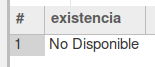
\includegraphics[width=.9\linewidth]{img/1.png}
\end{center}

\subsubsection*{Código}
\label{sec:org8e98765}
\\ \lstinputlisting{./src/P8.asm}

\section*{Conclusiones y comentarios}
\label{sec:org4772033}
Las operaciones con bits son más complicadas para nosotros porque estamos acostumbrados a trbajar 
con los valores decimales, sin embargo la compurtadora trabaja mas facilmente en binario por lo que 
para ganar mas velocidad de ejecucion podemos utilizar estas operaciones, quiza unos pocos 
cientos de veces no es justificacion para poder justificar usar ASM pero millones haga alguna 
diferencia significativa.


\section*{Referencias}
\label{sec:orgfb7582d}
\begin{description}
\item[{Bitshifting to multiply an integer by 10}] \url{https://stackoverflow.com/a/10758005}
\end{description}
\end{document}
